\documentclass[11pt,a4paper]{scrartcl}

% Pakete
\usepackage[english]{babel}
\usepackage[UKenglish]{isodate}
\usepackage{xcolor}
\usepackage{graphicx}
\usepackage{amsmath}
\usepackage{amssymb}
\usepackage{nicefrac}
\usepackage[utf8]{inputenc}
\usepackage{siunitx}
\sisetup{
output-decimal-marker={.},
exponent-product=\cdot }
\usepackage{esvect}
\usepackage{eqnarray}
\usepackage{placeins}
\usepackage{scrpage2}
\usepackage{nameref}
\usepackage{upgreek}
\usepackage{caption}
\usepackage{subcaption}
\usepackage{bm}
\usepackage{mwe}
\usepackage{tcolorbox}
\usepackage{listings}
\usepackage{xstring}
\usepackage{stringstrings}
\usepackage{floatflt}
\usepackage{pgfplots}
\usepackage{tikz}


% Custom colors
\definecolor{deepblue}{rgb}{0,0,0.5}
\definecolor{deepred}{rgb}{0.6,0,0}
\definecolor{deepgreen}{rgb}{0,0.5,0}
\DeclareFixedFont{\ttb}{T1}{txtt}{bx}{n}{12} % for bold
\DeclareFixedFont{\ttm}{T1}{txtt}{m}{n}{12}  % for normal

% tikz
\usetikzlibrary{arrows}

% caption setup
\captionsetup[subfigure]{labelformat=simple, labelsep=colon}
\renewcaptionname{english}{\figurename}{Fig.}
\renewcommand{\thesubfigure}{\arabic{figure}.\arabic{subfigure}}
\renewcommand{\thesubtable}{\arabic{table}.\arabic{subtable}}

% Listning Einstellungen
\lstloadlanguages{python}       % Default highlighting set to "python"
\DeclareCaptionFont{white}{\color{white}}
\DeclareCaptionFormat{listing}{%
  \parbox{0.99\textwidth}{\colorbox{gray}{\parbox{0.99\textwidth}{#1#2#3}}\vskip+5pt}}
\captionsetup[lstlisting]{format=listing, labelfont=white, textfont=white}
\lstset{frame=lrb,xleftmargin=\fboxsep,xrightmargin=-\fboxsep}
\pagestyle{empty}
\lstset{escapeinside={<@}{@>}}
\lstdefinestyle{MyPythonStyle}{
		language=Python,
		numbers=left,
		breaklines=true,
		basicstyle=\ttm,
		otherkeywords={self},             % Add keywords here
		keywordstyle=\ttb\color{deepblue},
		emph={MyClass,__init__},          % Custom highlighting
		emphstyle=\ttb\color{deepred},    % Custom highlighting style
		stringstyle=\color{deepgreen},
		frame=tb,                         % Any extra options here
		showstringspaces=false            % 
		}
\lstdefinestyle{MyCStyle}{
		language=C,
		numbers=left,
		tabsize=4,
		breaklines=true,
		basicstyle=\ttm,
		otherkeywords={self},             % Add keywords here
		keywordstyle=\ttb\color{deepblue},
		emph={MyClass,__init__},          % Custom highlighting
		emphstyle=\ttb\color{deepred},    % Custom highlighting style
		stringstyle=\color{deepgreen},
		frame=tb,                         % Any extra options here
		showstringspaces=false            % 
		}
\renewcommand{\lstlistingname}{Code block}
\renewcommand{\lstlistlistingname}{List of \lstlistingname s}

% Griechische Buchstaben vereinheitlichen
\renewcommand{\alpha}{\upalpha}
\renewcommand{\beta}{\upbeta}
\renewcommand{\gamma}{\upgamma}
\renewcommand{\delta}{\updelta}
\newcommand{\w}{\omega}
\newcommand{\la}{\lambda}

% Eigene mathematische Kommandos
\newcommand{\dd}{\text{d}} 							% Differential
\newcommand{\p}{\partial} 								% Partielles Differential
\newcommand{\D}{\Delta} 								% Fehler / Laplace
\newcommand{\order}[1]{\mathcal{O}\left( #1 \right)}
\newcommand{\abs}[1]{\left| #1\right|} 					% Betrag
\newcommand{\Max}[1]{\max \left\lbrace #1\right\rbrace} % max{}
\newcommand{\Min}[1]{\min \left\lbrace #1\right\rbrace} % min{}
\newcommand{\diff}[2]{\frac{\text{d} #1}{\text{d} #2}}	% Ableitung
\newcommand{\pdiff}[2]{\frac{\partial #1}{\partial #2}} % Partielle Ableitung
\newcommand{\errprop}[2]{\left| \frac{\partial #1}{\partial #2}\right| \cdot \Delta #2}
														% Fehlerfortpflanzung
\newcommand{\rel}[1]{\frac{\Delta #1}{#1}}				% Relativer Fehler

% Eigene trigonometrische Funktionen
\newcommand{\Exp}[1]{\text{exp}\left( #1 \right)}		% exp()
\newcommand{\Ln}[1]{\text{ln}\left( #1 \right)}			% ln()
\newcommand{\Log}[1]{\text{log}\left( #1 \right)}		% log()
\newcommand{\Sin}[1]{\text{sin}\left( #1 \right)}     	% sin()
\newcommand{\Cos}[1]{\text{cos}\left( #1 \right)}		% cos()
\newcommand{\Sinz}[1]{\text{sin}^2\left( #1 \right)}	% sin^2()
\newcommand{\Cosz}[1]{\text{cos}^2\left( #1 \right)}	% cos^2()
\newcommand{\Tan}[1]{\text{tan}\left( #1 \right)}		% tan()
\newcommand{\Asin}[1]{\text{asin}\left( #1 \right)}		% asin()
\newcommand{\Acos}[1]{\text{acos}\left( #1 \right)}		% acos()
\newcommand{\Atan}[1]{\text{atan} \left( #1 \right)}	% atan()

% Eigene Vektor Kommandos
\newcommand{\tovec}[2]{\begin{pmatrix}#1\\ #2\end{pmatrix}}	% 2D-Vektor
\newcommand{\trvec}[3]{\begin{pmatrix}#1\\ #2\\ #3\end{pmatrix}}	% 3D-Vektor	
\newcommand{\ovec}[1]{\boldsymbol{#1}}

% Eigene Referenz-Kommandos
\newcommand{\eref}[1]{(\ref{#1})}						% Gleichungen
\newcommand{\sref}[2]{\subref{#2}}						% Unterabbildungen
\newcommand{\kref}[1]{\ref{#1} \glqq\nameref{#1}\grqq}  % Kapitel
\newcommand{\lref}[1]{$[#1]$}							% Quellen: \newcommand{\lit}{1} => \lref{\lit}

% listing commandos
\newcommand{\listfile}[7][MyPythonStyle]{
\lstinputlisting[linerange={#4-#5}, firstnumber=#4, caption={#6} \hfill script:  \lstinline@#3@, label=#7, style=#1]{#2}}
% arguments:
% \listfile[style]{location/filename}{filename}{firstline}{lastline}{title}{label}
% Imports code from a file 
% You will not have to escape the filename, but the title
% style is an optional argument.

% commands for this task
\newcommand{\ua}{AU}
\newcommand{\vecx}[1]{\ovec{x}^{(#1)}}
\newcommand{\vecv}[1]{\ovec{v}^{(#1)}}
\newcommand{\veca}[1]{\ovec{a}^{(#1)}}
\newcommand{\vecF}[1]{\ovec{F}^{(#1)}}
\newcommand{\vecr}[1]{\ovec{r}^{(#1)}}
\newcommand{\nx}[1]{x^{(#1)}}
\newcommand{\nv}[1]{v^{(#1)}}
\newcommand{\na}[1]{a^{(#1)}}
\newcommand{\nm}[1]{m^{(#1)}}
\newcommand{\nF}[1]{F^{(#1)}}
\newcommand{\nr}[1]{r^{(#1)}}


% Kopf-/Fusszeile
\pagestyle{scrheadings}
\clearscrheadfoot
\chead{Simulation Methods in Physics I}
\ihead{Worksheet 2}
\ohead{\today}
\ofoot{\pagemark}
\ifoot{Michael Marquardt}

\begin{document}

% Titelseite
\begin{titlepage}

\ \\ \ \\ \ \\

\center\textbf{
\begin{large}
Simulation Methods in Physics I
\end{large} \\ \ \\
\begin{Large}
Worksheet 2: Statistical Mechanics and Molecular Dynamics
\end{Large}}   \\ \ \\
\ \\ \ \\

\begin{tabular}{lll}
Students: &Michael Marquardt &Cameron Stewart\\ 
matriculation numbers: &3122118 &3216338\\
\end{tabular}



\end{titlepage}

% Inhaltsverzeichnis
\tableofcontents
\newpage

% -------------------------------------- Begin Of Document ----------------------------------------

\section{Statistical Mechanics}

\subsection{Configurations of Thermodynamic Systems}

\begin{figure}[ht]
\centering
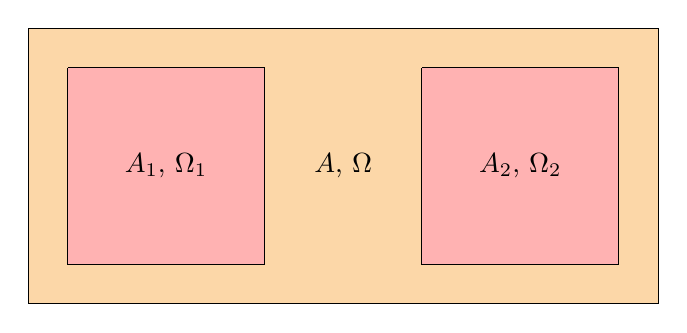
\begin{tikzpicture}
	\filldraw[fill=yellow!50!red!30!white]
		(0,0) -|(8,-3.5) -| (0,0);
	\filldraw[fill=red!30!white]
		(0.5,-0.5) -| (3,-3) -| (0.5,-0.5)
		(5,-0.5) -| (7.5,-3) -| (5,-0.5);
	\draw	
		(4,-1.75) node{$A$, $\Omega$}
		(1.75,-1.75) node{$A_1$, $\Omega_1$}
		(6.25,-1.75) node{$A_2$, $\Omega_2$};
\end{tikzpicture}
\caption{Thermodynamic System $A$ with a $\Omega$ possible configurations which is made up of the two Systems $A_1$ and $A_2$.}
\label{sysA}
\end{figure}

Figure \ref{sysA} shows a thermodynamic System $A$ which consists of two subsystems $A_1$ and $A_2$. 
Thereby the system $A_1$ has $\Omega_1=10^{31}$ and $A_2$ $\Omega_2=10^{28}$ possible configurations. 
The number of possible configurations $\Omega$ of the combined system $A$ therefore is the product of $\Omega_1$ and $\Omega_2$:
\begin{align}
\Omega 
	=&\; \Omega_1\cdot\Omega_2 
	= 10^{31+28} = 10^{59}
	\label{omega}
\end{align}

The entropy of such a system is $S=k_B \ln \Omega$, where $k_B=\SI{1.38E-23}{\joule\per\kelvin}$ is the Boltzmann constant. 
Therefor the entropies of $A$, $A_1$ and $A_2$ are:
\begin{align}
S_1 
	=&\; k_B\cdot \ln\Omega_1 
	= 31 k_B\cdot\ln 10  
	= \SI{9.850E-22}{\joule\per\kelvin}
	\label{S1}\\
S_2 
	=&\; k_B\cdot \ln\Omega_2 
	= 28 k_B\cdot\ln 10 
	= \SI{8.897E-22}{\joule\per\kelvin}
	\label{S2}\\
S 
	=&\; k_B\cdot \ln\Omega 
	= k_B\cdot\Ln{\Omega_1\cdot\Omega_2} 
	= k_B\cdot\ln\Omega_1+k_B\cdot\ln\Omega_2
	\nonumber\\
=&\; S_1+S_2 
	= 59 k_B\cdot\ln 10 
	= \SI{18.748E-22}{\joule\per\kelvin}
	\label{S}
\end{align}

As you can see, the entropy of the combined system is the sum of its sybsystems entropies.\\

\subsection{Isothermal Change of States}

Consider a volume $V_0=\SI{1}{\metre\cubed}$ of the nearly ideal gas neon at a pressure $p_0=\SI{1}{atm}=\SI{1013.25}{\hecto\pascal}$ and temperature $T=\SI{298}{\kelvin}$. 
Now the Volume of this gas is expanded isothermal by $\SI{1}{\percent}=f_V-1$. 
For an ideal 1-atomic gas the intrinsic energy is $U=\frac{3}{2}Nk_BT$. 
Because of this $U$ does not change through an isothermal process.
At least we can use the first principle of thermodynamics \eref{1HS} and the ideal gas law \eref{id} in order to derive the the factor $f_\Omega$ by which the number of possible states $\Omega$ increase. 

\begin{align}
\D U 
	=&\; \D Q + \D W
	\label{1HS}\\
pV 
	=&\; Nk_BT
	\label{id}\\
\D T 
	=&\; 0 
	\ \ \Rightarrow \ \ \D U 
	= \frac{3}{2}Nk_B\cdot \D T
	= 0
	\label{kons}\\
\dd S 
	=&\; \frac{\dd Q}{T} 
	\stackrel{\eref{1HS}}{=} \frac{\dd U-\dd W}{T} 
	\stackrel{\eref{kons}}{=} \frac{p}{T}\dd V 
	\stackrel{\eref{id}}{=} \frac{Nk_B}{V}\dd V 
	&&|\int
	\label{dS}\\
\int_{S_0}^{S_1} \dd S
	=&\; \int_{V_0}^{V_1}\frac{Nk_B}{V}\dd V
	\label{sint}\\
\D S 
	=&\; Nk_B\cdot\left(\Ln{V_1}-\Ln{V_0}\right) 
	=\frac{p_0V_0}{T}\cdot\Ln{\frac{V_0+\D V}{V_0}}
	\label{DS}\\
k_B\cdot \Ln{\frac{\Omega_0+\D \Omega}{\Omega}} 
	=&\;\frac{p_0V_0}{T}\cdot\Ln{\frac{V_0+\D V}{V_0}} 
	&&|:k_B
	\label{SO}\\
\Ln{f_\Omega} 
	=&\; \frac{p_0V_0}{k_BT}\cdot\Ln{f_V} 
	=\Ln{f_V^{\frac{p_0V_0}{k_BT}}} 
	&&|\exp
	\label{lnO}\\
f_\Omega 
	=&\; f_V^{\frac{p_0V_0}{k_BT}} 
	= f_V^N 
	= 29.5^{1/k_B} 
	\rightarrow \text{overflow}
	\label{Omega}
\end{align}

This is an incredible high number. 
This shall show that only a little more space for our simulation increases the number of possible staes with the power $N = \frac{p_0V_0}{k_BT}\approx\SI{41}{\mole}$ (number of particles). 

\subsection{Isochoral Change of States}

The considered system contains $N=\SI{1}{\mole}$ of particles at a temperature of $T_0=\SI{400}{\kelvin}$. Now an energy of $\D U =\SI{100}{\kilo\joule}$ is added to the system. We again want to figure out $f_\Omega$.
\begin{align}
\D V 
	=&\; 0
	\ \ \Rightarrow \ \ \D W 
	= -p \D V
	= 0
	\label{kons2}\\
\dd S
	=&\; \frac{\dd Q}{T}
	\stackrel{\eref{1HS}}{=} \frac{\dd U}{T}
	\label{dS2}\\
\dd U 
	=&\; \frac{3}{2}k_BN\cdot\dd T
	\ \ \ \text{(ideal gas)}
	\label{idU}\\
f_T 
	=&\; \frac{T_0+\D T}{T_0} 
	=1+\frac{2\D U}{3k_BNT_0}
	\label{fT1}\\
=&\; 21.06
	\label{fT2}\\
\dd S
	=&\; \frac{3k_BN}{2T}\dd T
	&&|\int
	\label{dSdT}\\
\int_{S_0}^{S_1} \dd S
	=&\; \int_{T_0}^{T_1}\frac{3k_BN}{T}\dd T
	\label{sint2}\\
k_B\cdot\Ln{f_\Omega}
	=&\; \frac{3}{2}k_BN\cdot\left(\Ln{T_1}-\Ln{T_0}\right) 
	= \frac{3}{2}k_BN\cdot\Ln{f_T}
	&&|:k_B\ |\exp
	\label{DO2}\\
f_\Omega 
	=&\; f_T^{\frac{3}{2}N}
	=21.06^{\frac{3}{2}\SI{}{\mole}}
	\rightarrow \text{overflow}
	\label{fO2}
\end{align}

As you can see, this number is also very large. The number of possible states increases with a factor to the power $\frac{3}{2} N = \frac{3}{2}\SI{}{\mole}$.

\subsection{Thermodynamic Variables in the Canonical Ensemble}

Helmholtz free energy:
\begin{align}
F 
	=&\; U\left( S(N,V,T),V,N\right) -T\cdot S\left( T,V,N\right) 
	=-k_BT\cdot\Ln{Z(T,V,N)}
	\label{helm}
\end{align}

From equation \eref{helm} we can derive the intrinsic energy $U$, the pressure $p$ and the entropy $S$. Therefor we use $\pdiff{U}{S}=T$.
\begin{align}
\pdiff{F}{V} 
	=&\; \pdiff{U}{S}\pdiff{S}{V}+\pdiff{U}{V}-T\pdiff{S}{V}
	=-p(T,V,N)
	\label{hp}\\
p(T,V,N) 
	=&\; \frac{k_BT}{Z(T,V,N)}\cdot\pdiff{Z}{V}(T,V,N)
	\label{hp2}\\
\pdiff{F}{T} 
	=&\; \pdiff{U}{S}\pdiff{S}{T}-T\pdiff{S}{T}-S
	=-S(T,V,N)
	\label{hS}\\
S(T,V,N) 
	=&\; \frac{k_BT}{Z(T,V,N)}\cdot\pdiff{Z}{T}(T,V,N)
	\label{hS2}\\
U(T,V,N) 
	=&\; T\cdot S(T,V,N) + F(T,V,N)
	\label{hU}\\
=&\; T\cdot S(T,V,N)-k_BT\cdot\Ln{Z(T,V,N)}
	\label{hU2}	
\end{align}

\subsection{Ideal Gas}

The canonical partition function if an ideal gas is:
\begin{align}
Z(T,V,N)
	=&\; \frac{V^N}{\la^{3N}N!}
	&\la 
	=&\; \sqrt{\frac{h^2\beta}{2\pi m}}
	&\beta 
	=&\; \frac{1}{k_BT}
	\label{Zid}
\end{align}

Now we calculate the Helmholtz free energy $F$ \eref{helm} for this partition function $Z$.
\begin{align}
F(T,V,N)
	=&\; -k_BT\cdot\Ln{\frac{V^N}{\la^{3N}N!}}
	\label{f1}\\
	=&\; -k_BT\cdot\left(N\cdot\Ln{\frac{V}{\la^{3}}}-\Ln{N!}\right)
	\label{f2}\\
	\stackrel{N>10^3}{=}& -k_BTN\cdot\left(\Ln{\frac{V}{\la^{3}N}}+1\right)
	\label{f3}\\
=&\; -k_BTN\cdot\left(\Ln{\frac{V}{N}\left(\frac{2\pi mk_BT}{h^2}\right)^{3/2}}+1\right)
	\label{f4}
\end{align}

The last step is to derive an expression for the heat capacity at constant volume $C_V$. 
\begin{align}
C_V 
	=&\; \left(\diff{Q}{T}\right)_V
	=\left(\diff{U}{T}\right)_V
	\stackrel{\eref{hU}}{=} \left(\diff{(T\cdot S+F)}{T}\right)_V
	\label{cv1}\\
S(T,V,N)
	\stackrel{\eref{hS2}}{=}&\; -\pdiff{F}{T}
	\label{fs1}\\
\stackrel{\eref{f4}}{=}&\; \pdiff{ }{T} k_BTN\cdot\left(\Ln{\frac{V}{N}\left(\frac{2\pi mk_BT}{h^2}\right)^{3/2}}+1\right)
	\label{fs2}\\
=&\; k_BN\cdot\left(\Ln{\ldots}+1\right)
	+ \frac{3}{2}k_BN\cdot\left(\frac{2\pi mk_BT}{h^2}\right)^{3/2}\cdot\left(\frac{2\pi mk_BT}{h^2}\right)^{-3/2}
	\label{fs3}\\
=&\; -\frac{F}{T} + \frac{3}{2}k_BN
	\label{fs4}\\
C_V
	\stackrel{\eref{fs4}}{=}&\; \left(\diff{(-T\cdot\frac{F}{T}+\frac{3}{2}k_BNT+F}{T}\right)_V
	=\left(\diff{}{T}\frac{3}{2}k_BNT\right)_V
	\label{cv2}\\
=&\; \frac{3}{2}k_BN
	\label{cv3}
\end{align}

\section{Molecular Dynamics: Lennard-Jones Fluid}
In this worksheet we will simulate a simple Lennard-Jones fluid using Molecular Dynamics.  We begin by implementing the Lennard-Jones (LJ) potential and force in python and simulate a few particles as "billards." We will move on to simulating a LJ fluid using periodic boundary conditions and random initial velcities. We then compare the run times for this system using implementations using python, C, and cython. Finally, we include cell lists and Verlet lists in order to further improve our efficiency.
\subsection{Lennard Jones Potential}
The LJ potential is originally a model used to represent a system of noble gas particles and consists of a hard core repulsion as well as a longer ranged attractive potential due to the dipole-dipole interaction. At longer ranges the potential is nearly zero. It is given by
\begin{equation}
V_\mathrm{LJ}(r) = 4\epsilon\left(\left(\frac{\sigma}{r}\right)^{12} - \left(\frac{\sigma}{r}\right)^6\right).
\end{equation}
\subsection{Reduced Units}
We may define a set of dimensionless reduced units because the LJ potential is of the general form
\begin{equation}\label{genpot}
U(r) = \epsilon \phi(\sigma/r)
\end{equation}
where $\sigma$ and $\epsilon$ are constants and $\phi$ is smooth and differentiable. We use
\begin{equation}
x^* = x/\sigma,\quad V^* = V/\sigma^3, \quad T^* = k_\mathrm{B} T/\epsilon,\quad p^* = p\sigma^3/\epsilon.
\end{equation}
The law of corresponding states claims that any system interacting with an potential such as \ref{genpot} is described by the same equation of state. We may therefore simulate at $/epsilon = /sigma = 1.0$ without any loss of generality.

With the help of numpy, we implement the LJ potential in the following way:
\listfile{../src/ljlib.py}{/src/ljlib.py}{10}{13}{LJ Potential}{ljpotential}
The force due to this potential is simply given by the negative gradient and is implemented as:
\listfile{../src/ljlib.py}{/src/ljlib.py}{15}{19}{LJ Force}{ljforce}
The output of these functions for values from 0.85 to 2.5 can be seen in Fig. \ref{fig:lj}.
\begin{figure}[h]
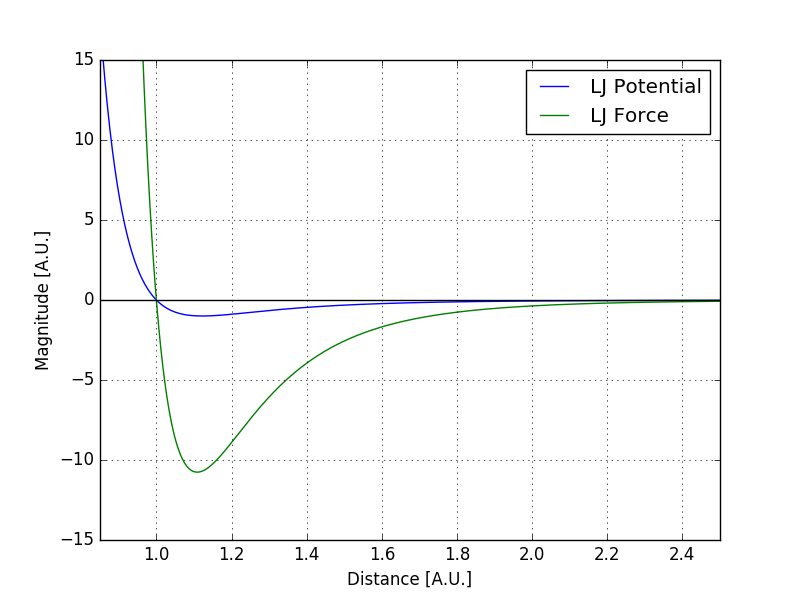
\includegraphics[width=0.7\linewidth]{../fig/ljplot.png}
  \centering
  \caption{Output of the compute\_lj\_potential and compute\_lj\_force functions.}
\label{fig:lj}
\end{figure}
\subsection{Lennard-Jones Billards}
We would now like to use this potential to run an MD simulation.We use the velocity verlet integrator to run the MD. Our first simulation will place 5 particles by hand and integrate until $t = 20.0$ with a timestep of $dt = 0.01$. We begin with a supplied template and simply import the library created in the previous task.  
\listfile{../src/ljbillards.py}{/src/ljbillards.py}{1}{3}{Import ljlib.py}{imports}
We can use VMD in order to visualize the simulation once we've run the program. A still shot from our simulation can be seen in Fig. \ref{fig:vmd}.
\begin{figure}[h]
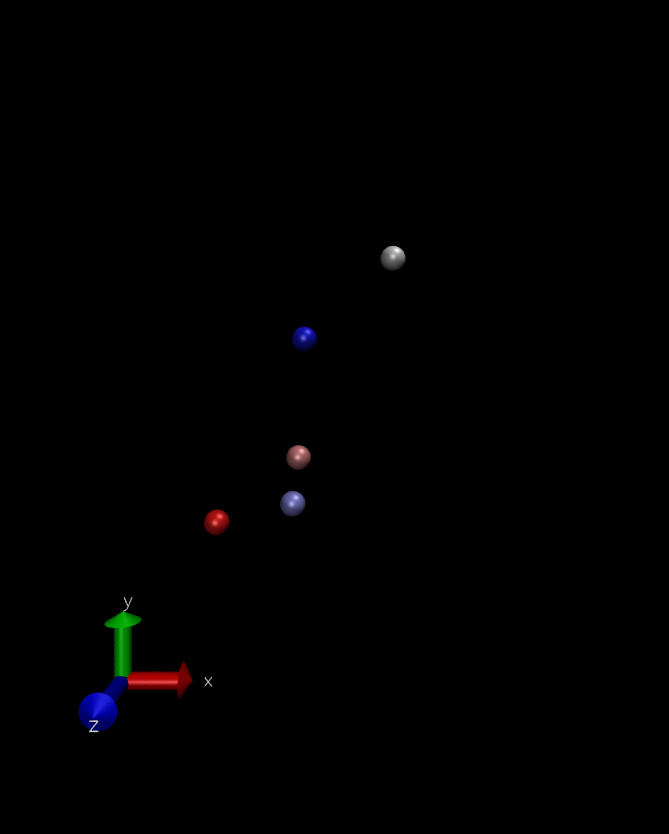
\includegraphics[width=0.7\linewidth]{../fig/vmdscene.png}
  \centering
  \caption{A snapshot of the LJ billards simulation}
\label{fig:vmd}
\end{figure}
In the original simulation, the first (not zeroth) particle did not collide with the fourth. We moved the fifth particle slightly south in order to correct this and the trajectory can be seen in Fig. \ref{fig:bplot}. Another feature of this trajectory is that the second and third particles do not behave like billard balls at all. This is due to the attractive part of the LJ potential.
\begin{figure}[h]
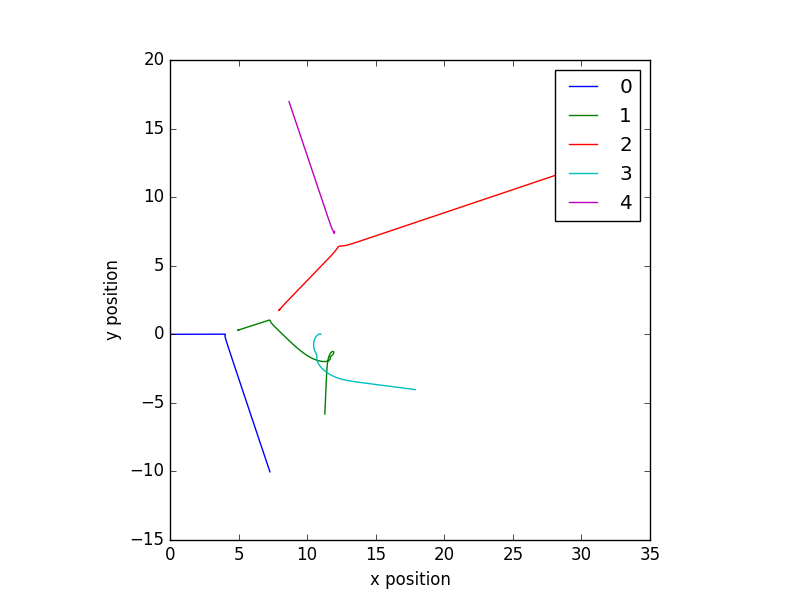
\includegraphics[width=0.7\linewidth]{../fig/billardplt.png}
  \centering
  \caption{Billard trajectory with modified initial conditions}
\label{fig:bplot}
\end{figure}
\subsection{Periodic Boundary Conditions}
Because computers have limited resources and computing power, we can never simulate a full system. Rather we simulate a much smaller system. Unfortunately, if we had only a few particles in a boundless space, they would escape to infinity and no longer interact. We can't simply add walls because we must then account for surface effects. We can solve this problem by using periodic boundary conditions (PBC).  Images of our central box essentially extend infinitely in every direction. We now have an infinite volume $V$ and particle number $N$ but we may prescribe a density $\rho = N/V$.
\subsubsection{Long and Short Range Interactions}
One problem with an infinite number of particles is that long range interactions become hard to model since we must compute an infinite number of interactions. Fortunately, LJ is essentially short ranged and we can define a cutoff distance as follows.

\begin{equation*}
V^`_\mathrm{LJ}(r)=\begin{cases}
V_\mathrm{LJ}(r) - V_\mathrm{LJ}(r_\mathrm{cutoff}), & r \leq r_\mathrm{cutoff}\\
0, & \text{else}
\end{cases}
\end{equation*}
We implent this for both the LJ potential and force as
 \listfile{../src/ljlib.py}{/src/ljlib.py}{21}{35}{LJ Cutoff}{cuttoff}
We use a value of $2.5$ for $r_\mathrm{cutoff}$.
\subsubsection{Minimum Image Convention}
If we use a cutoff range that is less than the length of our box $L$ then we only have to compute the interaction between the closest image of the particles. All other images will be too far to interact. Knowing this, we can implement pbc by simply calculating the minimum image distance and using that distance to calculate the forces. Our particles will then freely propogate outof the box while still experiencing the correct force. When looking at the trajectory in VMD or in python we can then simpy wrap the particle locations back to the first box to see the true trajectories. The following code block shows how the minimum image is calculated:
 \listfile{../src/ljbillards1.py}{/src/ljbillards1.py}{54}{57}{Minimum Image}{image}
 The compute\_forces function was modified as well.
  \listfile{../src/ljbillards1.py}{/src/ljbillards1.py}{5}{19}{PBC Forces}{pbcforces}
We tested the pbc by setting up two particles with the following initial conditions:
 \listfile{../src/ljbillards1.py}{/src/ljbillards1.py}{67}{75}{Initial Conditions}{init}
The trajectory can be seen in Fig. \ref{fig:pbc}. 
\begin{figure}[h]
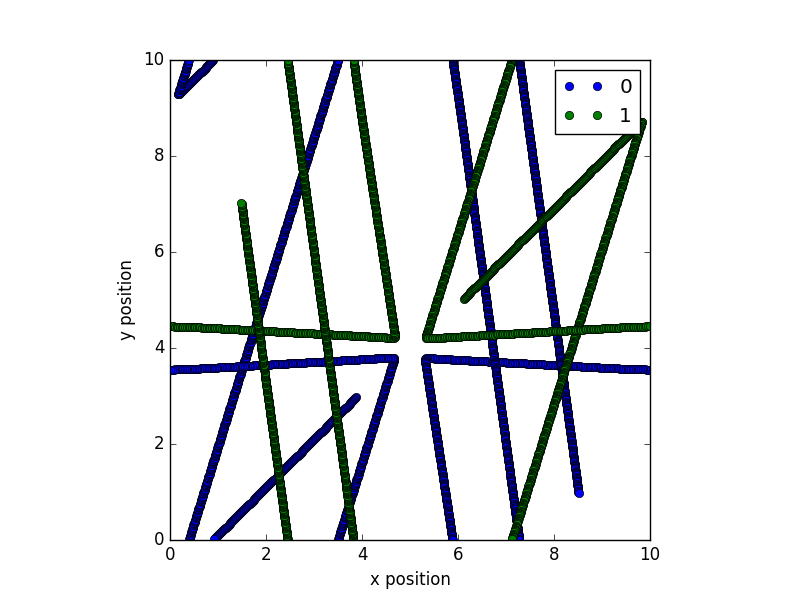
\includegraphics[width=0.7\linewidth]{../fig/pbcplot.png}
  \centering
  \caption{Billard trajectory with modified initial conditions}
\label{fig:pbc}
\end{figure}
\subsection{Lennard-Jones Fluid}
\subsubsection{Pure Python}
We now inherit a nice python program to simulate an LJ fluid with periodic boundary conditions. We have only to import {\tt ljlib.py}, compute the size of the system, and place the particles programatically as shown in the following code block.
 \listfile{../src/ljfluid.py}{/src/ljfluid.py}{81}{88}{Particle Placement}{place}
We then ran the simulation with $n = {3, 4, 5}$ particles per side for $t = 1.0$ and $dt = 0.01$ and measured the time taken to complete the simulation. We recorded times of 1.472, 5.328, and 16.704 seconds respectively.
\subsubsection{Pure C/C++}
Similar to the previous task we were given a template to modify. In this case we needed to implement the compute\_energy() function.
 \listfile{../src/ljfluid.cpp}{/src/ljfluid.cpp}{73}{91}{Compute Energy}{computeenergy}
We then ran the simulation for $n = {5,6,7,8,9,10,11,12}$ and measured the computation time. For $n=5$, a time of 0.188 seconds was measured. Almost 10 times faster than python. The data along with a fit of the obvious quadratic trend is included in Fig. \ref{fig:cpp}.
\begin{figure}[h]
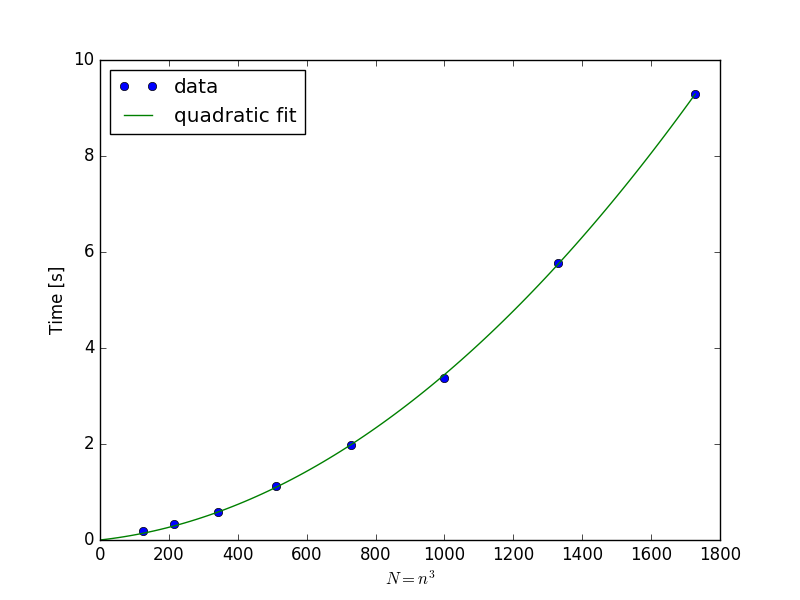
\includegraphics[width=0.7\linewidth]{../fig/fit.png}
  \centering
  \caption{Plot of number of particles vs computing time for the C++ implementation along with a quadratic fit.}
\label{fig:cpp}
\end{figure}
\subsection{Cython}
Finally we will use cython as an interface between python and C so that the time intensive code is written in C and the control is done with python. We copied the compute\_energy() function from the previous task into the supplied template, lines 10 1nd 21 through 24 were uncommented in {\tt /src/cython1/lj.pyx}, and lines 84 through 87 were uncommented in {/tt /src/cython1/ljfluid.py}.

\end{document}
